
\chapter{Programming Model}\label{ch:prog}

\squo{POKE: Fear of failure is a poor reason not to try.}{\emph{Outer Wilds}}

\begin{chabstract}
    This chapter will discuss the programming model of Twizzler at a higher level than operating system interfaces,
    including object layout, safety, and lifetime.
\end{chabstract}

While the direct interfaces presented by the operating system are important, most programmers will not directly interact
with them. Instead, they will use higher-level interfaces provided by a standard set of Twizzler libraries. We will now
take a look at some of the aspects of writing programs that use objects on Twizzler. Note, though, that we are still
leaving a lot up to specific language runtimes and instead of being doctrinaire about all aspects of the system, we
prefer to allow flexibility. An example of this, which we will explore in more detail in this chapter, is not
preventing ``persistent to volatile'' references at a system level, and instead relying on higher-level runtimes to
enforce such things.

\section{Object Layout}
Recall that objects are, fundamentally, a ``bag of bytes'', all identified via an ID and an offset, with some areas
pre-defined, for example, the FOT.
Objects in Twizzler often have a header at the object's base, the contents of which depend on what
the object contains. Often these headers have pointers to other data in the object, and describe the
type of the object. For example, in our evaluation we implement a red-black tree in an object. The
header contains some basic information about the tree as well as a pointer to the root node. Placing
headers at the object's base gives applications a ``starting point'' that they can use to start
accessing object data. Twizzler provides a dedicated function to get a pointer to an object's
header, called \texttt{obj\_base}.

Note that the base address of an object is \emph{not} at offset $0$, but instead one page up, so that we
can still trap NULL pointers. If this were not the case, a pointer value of $0$ would still be a valid
pointer, and we want to remain backwards compatible with the assumption that a NULL pointer has
integer value $0$. The bottom page of an object is unmapped by Twizzler, allowing NULL pointer
dereferences to be trapped by the kernel.

While objects are flat, contiguous regions of memory, different applications may want to organize
that memory in different ways. Some objects, such as \texttt{views} are largely interpreted as an
array, but sometimes applications need to explicitly allocate and deallocate memory within an object.
Twizzler provides an API to allocate and free units of memory from application-specified regions
within objects. We make use of this in our red-black tree code, where new nodes are allocated out of
the object using this API.

\begin{SCfigure}
    \centering
    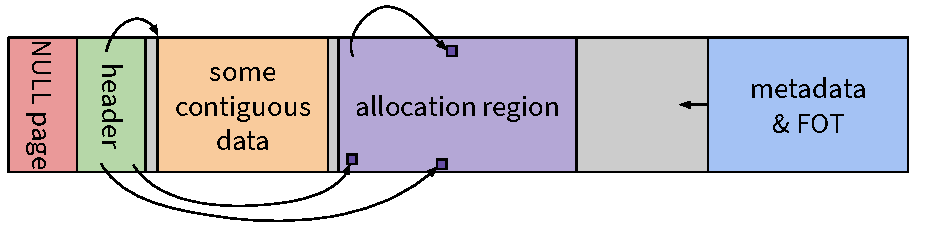
\includegraphics[width=\linewidth]{fig/typobj}
    \caption[Typical object layout]{A typical object layout. The header, contiguous region, and allocation region are all
        optional, however most objects will have a header. This object contains a number of internal
        pointers between regions. The metadata region (which includes the FOT) grows downward.}
    \label{fig:typobj}
\end{SCfigure}

Figure~\ref{fig:typobj} shows a typical object in Twizzler. The NULL page is always present to trap
NULL pointers, and is followed by a header. The application setting up this object may have a region
of some contiguous data, such as some strings, or an array, and may point to it from the header.
The object may have a region setup for allocation so that a future application using this
object can easily allocate and free memory when manipulating the object. Finally, the FOT and
metadata regions start at the top of the object and grow downwards.

\paragraph{Ensuring Base Type Properties}

When accessing persistent or shared data for the first time, it's necessary to specify the type of the data. For
objects, this means we need to specify the type of the header, as objects are typed by their header, also called the
object ``base''. While in C the function that gives access to the base returns a \texttt{void *}, the function in Rust
returns a reference to the specified base type. From there, any other data accessed traverses data structures that use
the type system. Twizzler's invariant pointers' Rust implementation is typed, and the mutability rules ensure that our
transaction engine properly ensures transactional properties, so any data to which we can get a reference is
well-typed as long as the header of the object is well-typed.

To ensure this, we encode, in the object's metadata, a pair of 64~bit numbers that refer to a unique ID of the header
type\sidenote{This is currently allocated manually, though we plan to automatically generate the IDs via procedural
    macros in the future.} and a version number. When code tries to access the header, we do a one-time check to see if the
recorded ID and version match the ID and version from the type that we are supposed to return. If they fail to match, we
can return an error, and if they do match, then we know it's the correct type (up to collisions in the ID space, that is).

\section{The Flipside}

One aspect of programming for \NVM that is somewhat orthogonal to Twizzler's primary object model is considering what
effects writes will have to the actual physical media. This kind of consideration is common---we think about block
layouts and overwrites when considering differences between magnetic disk and SSDs---but for \NVM, we should ask what
the new device characteristics are, since
it is important that systems are optimized to leverage their
strengths and avoid stressing their weaknesses. We typically try to reduce writes to physical media, however with
\NVM it turns out that the number of \emph{bits flipped} may be the more important metric.

\NVMs such as PCM suffer from both wear and energy use when it must flip a stored bit. Applications such as IoT devices
cannot tolerate wear out and energy use as easily as other applications, and these devices make good targets for the
already dense and power efficient \NVM technologies.
Flipping a bit in PCM cells consumes $15.7\mathit{-}22.5\times$ more power than reading a
bit~\cite{dhiman_pdram:_2009,lee_architecting_2009,xiangyu_dong_nvsim:_2012,qureshi_scalable_2009}, and causes wear
(whereas reading causes comparatively little wear).
Thus, controllers can optimize by examining bits to determine which must actually change on a write~\cite{yang:iscas07}.
Of course, such an optimization is dependent on software, which issues the writes.
Reducing bit flips, an optimization goal that has yet to be
sufficiently explored, can both save energy and extend the life of \NVM, but we can optimize better by
designing software to reduce bit flips.

We examined a number of common data structures and strategies for how we can reduce bitflips caused
by data structure updates. This involved taking previously-known tricks like XOR linked lists~\cite{xorll} and
generalizing them to trees and hash tables, along with choices for bit packing and data layout, and modifying Gem5, a
system simulator, to count bit flips. We found that we could easily reduce a significant number of bits flipped in the
data structures we studied with little performance impact. Further details can be found in Appendix~\ref{app:bitflip}.


\section{Crash Consistency}
\label{sec:crash}

\Twizzler provides primitives for building crash-consistent data structures. At a low level,
it provides mechanisms for writing back cache-lines, appropriate fences, and basic transactions.
Applications use these primitives today outside of \Twizzler to build up larger, more complex support for
crash-consistent data structures.
%, thus we provide similar primitives.


\paragraph{Persistent Memory}

Programming against persistent memory has some advantages compared to programming against volatile memory and needing to
flush dirty pages to stable storage. Not only is it much faster, but failure-atomicity of an \NVM data structure can be
maintained by the application alone (if it so desires).
Our goal is to provide low level primitives without restricting programs or prematurely
prescribing particular solutions. There is a wealth of research on crash-consistent
data structures for
\NVM~\cite{condit:sosp09,coburn:asplos11,volos:asplos11,dulloor:eurosys14,narayanan:asplos12,ni:hotstorage18,ni:micro19,ogleari:hpca18,lu2014loose},
but it is still in flux. Of course, \Twizzler manages \emph{system} data structures,
such as FOT entries, views, \emph{etc.}, in a
crash-consistent manner using the aforementioned primitives, locking, and fencing.

\begin{SCfigure}
    \centering
    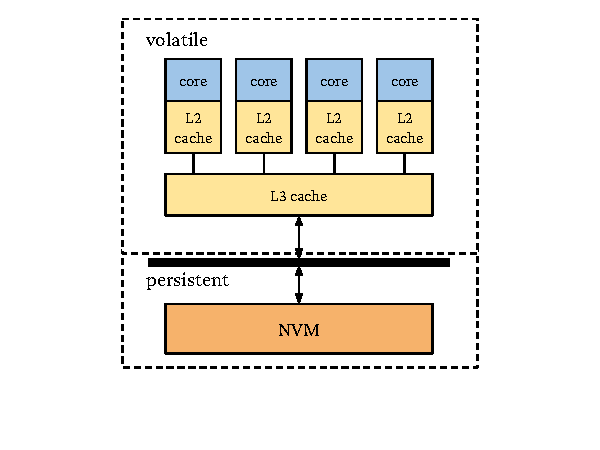
\includegraphics[width=\linewidth]{fig/vpdomains.pdf}
    \caption[Volatile and persistent domains]{Volatile and persistent domains. Once the memory controller has acknowledged the write, the system guarantees persistence of the write.}
    \label{fig:vpdomains}
\end{SCfigure}



At the time of writing, Intel systems handle \NVM by enabling a certain level of control over the cache system by
applications, notably via the \texttt{clwb} and fence instructions. Figure~\ref{fig:vpdomains} shows the boundary
between persistent and volatile domains in an abstracted CPU that operates roughly like how Intel's do. In this model,
any data stored in the cache is volatile, and will be lost if power is lost. Any data that makes it to the memory
controller (for which the memory controller acknowledges the write) is persisted. A small amount of internal residual
power is used by the persistent memory device to ensure the writes that reached the memory controller are stable.

With this model in mind, we can ensure failure atomicity in a rather inelegant manner if we use the \texttt{clwb}
instruction to ensure cache lines are flushed and the appropriate fence instructions to ensure durability, and end up
with a programming model reminiscent of multithreaded code using fences. We can abstract this a little bit to allow the
flushing of \emph{types} so as to avoid the programmer having to think entirely in cache lines. However, this still is a
lower level than most programmers likely want for ensuring safety. While Twizzler does provide a set of interfaces for
persisting data at this level, it also supports a basic transactional interface.


\paragraph{C Transactions Interface}
\Twizzler provides a transactional-persistent logging mechanism.
Programmers can write \texttt{TXSTART}/\texttt{TXEND} blocks to denote transactions and \texttt{TXRECORD}
statements to record pre-changed values, similar to the mechanism provided by
PMDK~\cite{libpmem}. If applications need more complex
transactions using different logging mechanisms, they can use libraries. \Twizzler's internal data
structures and \libcore's manipulation of object metadata is handled via a combination of these
transactions and cache-line writebacks.


\paragraph{Rust Transaction Interface}

The Rust interface to transactions is much safer than the C version, as it actually enforces various rules about type
safety, aliasing, and mutability. An example transaction block is written like,

\begin{lstlisting}[language=Rust]
    obj.tx(|tx| {
        let base = obj.base_mut(tx); // :&mut BaseType
        base.do_something();
    });
\end{lstlisting}

Here we start a transaction and get access to a transaction handle (\texttt{tx}). When we want to get a mutable
reference to part of the object, we must pass in a transaction handle, and the only way to get a transaction handle is
via the \texttt{tx} function. Thus we can enforce the aliasing rules for Rust inside the transaction framework.

\paragraph{Thread Restart}

\Twizzler provides a mechanism for restarting threads when power is restored following a crash.
Since views are persistent objects, all objects mapped during a thread's execution are known across
power cycles, and are mapped back in. The thread is then started at a special \texttt{\_resume}
entry point, allowing the program to handle the power failure in an application-specific manner.  Of
course, \emph{volatile} objects will be lost when power resumes, and thus any attempted access to
these objects will result in an exception. Applications that wish to resume after power failure
will need to be aware of and handle this. We do not wish to prescribe any restrictions
here---applications that want to place their heap in volatile memory for performance or security
reasons should be allowed to. We expect higher level support for applications to manage persistent
data, such as language support for persistent heaps, to make use of the features we provide, so
applications that want to resume can put resuming information in persistent objects.

The reason we choose to restart threads at a known, different entry point from normal application
start up is that in current systems, there is always volatile computation state (\eg registers, the
cache) that is lost when power is lost. Of course, in the future, systems may be able to prevent the
loss of more and more ephemeral computation state (with the logical extreme being perfect
resumability). In this case, the \texttt{\_resume} handler can be a simple stub that resumes the
execution exactly as left off. The more likely case, periodic checkpointing, can be similarly
handled, with the \texttt{\_resume} handler selecting the most recent valid check point to resume
from. The \texttt{\_resume} handler enables all of these solutions, thus remaining applicable across
hardware evolution.
\section{Memory Safety and Lifetimes}

One final aspect of objects is safety, that is, ensuring proper typing of memory and ensuring that object memory does
not leave a dangling reference behind. Twizzler accomplishes this via a combination of
some runtime checks, some kernel support for specifying lifetime relationships between objects, and some language
support.
%Notably, using the Rust bindings provides significantly more memory and type safety than the C bindings do.

\subsection{Object Types, Persistence, and Lifetime}

%% TODO ensure these types are consistent with previous chapter.
Applications need to be able to specify what \emph{type} of memory an object resides in. Currently,
we are operating on systems that contain both persistent \NVM and volatile DRAM as main memory, and
applications may want to make use of both of these memory types. Placing certain objects in DRAM,
for example, can result in performance improvements (\eg caching read-only objects) or security
improvements (\eg making temporary key material volatile). \Twizzler exposes this choice to
applications at object creation time, allowing them to specify the type of the object. At least two
types, \emph{volatile} and \emph{persistent}, are supported by default. As additional types of physical memory
are added to systems (\eg different kinds of \NVM with different properties, high-bandwidth memory,
\etc), applications may wish to have more fine-grained control over where objects are placed, and
\Twizzler's APIs allow such control. Objects can also be moved between types of memory after
creation, though this may be a time consuming operation as it involves copying potentially large
amounts of data.

By default, objects are persistent and live in kernel-managed \NVM or pager-managed storage unless they are marked as
volatile. If an object is volatile, it has a limited lifetime that is related to the power state of
the machine---as soon as power is lost or the system is rebooted all volatile objects disappear.
Note that \Twizzler removes the distinction between volatile and persistent objects for how
applications \emph{access} data, relying on higher-level language or library support and application
support for dealing with the limited lifetime of volatile objects.

The property of persistent versus volatile for objects differs from the concept of
ephemeral data. The ``volatile'' property places a physical restriction on the lifetime of an object (the machine's
power state), while the ``persistent'' property indicates that the object will exist until
explicitly deleted. Objects can also be long-lived or ephemeral independent of their persistence
property, since we use the term ``ephemeral'' to describe information, data, or state that has a
finite lifetime and is expected to ``go away''. While all volatile objects are ephemeral, the
reverse is not true---we may place ephemeral data in a persistent object to allow for recovery
after an unexpected power cycle. The ``persistent'' property of an object is a recorded piece
of information that the kernel associates with an object, but there is no such information for ephemeral
versus long-lived. Instead, we provide a mechanism for specifying a logical lifetime of objects
relative to one another with a mechanism called \emph{ties}, which we will discuss below.

\subsection{Object Ties and Logical Lifetime}

\iffalse
    Objects are, by default, persistent and live in kernel-managed \NVM. During creation, an object may
    be marked as ``volatile'', allowing the kernel to allocate memory for it from DRAM. This is useful
    for temporary application data that does not need to be persistent, such as stacks or volatile
    heaps. At any time, an object may be changed from volatile to persistent, or vice versa, but this
    may be a time consuming operation. Note that, although \Twizzler does distinguish between volatile
    and persistent objects (and allows applications to choose based on some policy what their objects
    are), \Twizzler removes the distinction between them when it comes to accessing the data.

    Throughout the paper, we use both terms ``volatile'' and ``ephemeral'' for different purposes.
    Volatile is a property of hardware---the data goes away when power is lost. We expose this meaning
    in objects that are marked as ``volatile'' to allow application to capitalize on the benefits of
    volatile memory (both performance and security). Ephemeral, more broadly, describes information,
    data, or state that has a finite lifetime and may ``go away''. This is in contrast to persistent
    data which has an ``infinite'' lifetime, and volatile data which has a finite lifetime tied to the
    power state of the machine. All volatile objects are ephemeral, while the reverse is not necessarily
    true (\eg an application may have some temporary state that it makes persistent to recover from a
    power cycle).
\fi

%An example of ephemeral data is temporary application data like a stack or a heap.
Applications in \Twizzler also have a lifetime; an application's job is typically to operate on
some persistent data while performing some computation before eventually exiting. Such an
application will likely use volatile objects to represent temporary computation state (\eg the
stack and heap, which are ephemeral). However, just assigning an object as volatile is insufficient
because there is a lifetime mismatch: the volatile object will live until the next reboot while the
application may exit before then or may even live and try to recover after a power cycle.
Manually deleting the volatile object when the application is done is also insufficient, as it does
not account for crashes where the application may be unable to clean up its state. Furthermore,
applications that wish to support recovery may make use of persistent stacks and heaps, thus these
objects would have to be persistent despite being ephemeral.

While we could provide a mechanism designed specifically for this ``system-level'' task,
where the kernel maintains a set of objects to automatically cleanup when an application exits, this
would require the kernel to have some understanding of what an ``application'' is. Furthermore, if
we generalize a solution to automatic cleanup, we can allow applications to make use of it for their
own purposes. For example, in \unix, it is common for programs to create and immediately unlink
files to ensure the system frees those resources when the program exits. We would like to reproduce
similar semantics here that also solves the lower level problem above of freeing application state
by assigning a lifetime to objects that is more expressive than simply ``volatile'' and
``persistent''.

\iffalse
    Applications need a mechanism to express the relative lifetime of objects in the system to ensure
    that a given object exists at least as long as another object. Specifying object lifetimes is
    commonly used to enable automatic cleanup. For example, in \unix, programs often create and
    immediately unlink files to ensure the system deletes them on exit. Similarly, a lot of ephemeral
    resources that applications typically use (\eg the stack, the heap) are formalized as objects in
    \Twizzler\sidenote{Formalizing these resources as objects both simplifies the programming
        environment model and allows them to be optionally persisted, allowing applications to resume their
        state after crashes.}.
\fi

In \Twizzler, object lifetime is expressed through \emph{ties}.
An object can be tied to another by invoking a system call that tells the kernel that
object \texttt{A} is tied to object \texttt{B}, after which the lifetime of \texttt{A} is
guaranteed to be at least that of \texttt{B}. The kernel will not fully delete object \texttt{A}, even if the
delete system call is invoked on it, until after \texttt{B} is fully deleted. An object may be tied
to a large (but finite) number of other objects and may also be \emph{untied} at any time. This
model of specifying object lifetime relative to others is similar to Rust~\cite{rust}, where
reference lifetime can be named so that the programmer can express lifetimes of objects relative to
each other. Note that object ties are not related to invariant pointers (discussed in more detail
in Chapter~\ref{ch:invariant}), and instead primarily provide a way to formalize automatic cleanup.


Object ties provide a convenient mechanism for applications to build data structures across
multiple objects without giving up easy cleanup if something goes wrong or if the ``root'' object is
deleted. \Twizzler also uses ties internally: when an object is created as copy-from an existing
object, it uses copy-on-write semantics, and thus internally marks the source object as tied to the
new object. We also tie ephemeral program state objects to threads (which are also represented by
objects) such that they are automatically cleaned up when a program exits. It is our expectation
that programmers will only rarely directly use ties. Instead, we expect that ties will
provide necessary features that higher-level programming language support for persistent memory can
use.

Note that object ties interact with the notion of volatile and persistent objects, because
volatile objects have an implicit \emph{maximum} lifetime---that of the next machine restart or
power loss. Tying volatile objects to volatile objects and persistent objects to persistent objects both act as
expected. Tying a persistent object to a volatile object is also semantically simple (persistent
objects already have an ``assumed lifetime'' that is longer than a volatile object). Tying a
volatile object to a persistent object, however, may seem somewhat nonsensical. However, \Twizzler
does still allow this because it has useful semantics: if an application creates a data structure
with some volatile component\sidenote{Since \Twizzler's kernel is not involved in reference
    creation, it cannot prevent such a reference from being created. We expect language support for
    persistent data structures to impose restrictions on applications in this regard, and the OS should
    not prematurely restrict how applications use volatile and persistent objects. Access to a volatile
    object that no longer exists after a reboot results in a simple access fault, mitigating security
    concerns.},
%\footnote{We will discuss the implications of creating references
%between volatile and persistent objects in \S~\ref{twz:pptr}.}
it may want to tie the lifetime of that volatile component to the
persistent component if the data structure is to be deleted. This use case (creating a persistent
object that we expect to delete) is not uncommon, particularly in applications designed to recover
partial computation after a crash. Note that, in this case, the maximum
lifetime of the volatile object is still in-play; after a power cycle, that object will no longer be
present, so tying a volatile object to a persistent object is somewhat dangerous.


\subsection{Safe Allocation}

As we discussed above, an object may optionally have a region within which we rely on an object memory allocator to
organize memory. However, when objects may be persisted or shared, there are some additional hazards to consider.

\begin{enumerate}
    \item \textbf{Crash Consistent}: The allocator must allow for power or application failures, and so
          all operations must be failure-atomic.
    \item \textbf{Leaked Memory}: Say we allocate some memory from an object. Let's consider the interface described
          by \texttt{malloc} and \texttt{free}. We can imagine a situation where an application allocates some memory, but
          before we manage to store the pointer anywhere, the power is reset. Or, alternatively, after a node is removed from,
          say, a list, but before the call to \texttt{free} is made, the power dies. In both cases the memory is leaked, and
          cannot be recovered without some application-specific \texttt{fsck}-like check.
    \item \textbf{Dangling Pointers}: Imagine that same scenario with freeing a node, but this time, the order of operations
          (remove node, then free) is not specified\sidenote{This could happen to improper use of transactions or persist
              barriers.}. Or, similarly, we allocate some memory and write a new node, and link it, but the order of operations is
          wrong again. Both of these cases result in writing a pointer to memory considered freed by the allocator.
\end{enumerate}

One might wonder if there concerns are specific to \NVM, where hardware persists behind a curtain, or more generally,
perhaps when we are flushing periodically to disk. Certainly we must worry about the above issues if hardware is
controlling persistence, but we still care even without \NVM. The \emph{semantics} of accessing an object are of sharing
it or not (recall from Chapter~\ref{ch:datacentric} that persistence \emph{is} sharing), and thus once it's shared it
could be in multiple places in space and/or time. We must, therefore, make allocation and resource acquisition, and
deallocation and reference removal failure-atomic. Consider a case where we interrupt an allocator operation after part
of the allocator state is persisted to disk and the power fails. The problems above still exist, even for persistent
objects stored on a disk or SSD.

To properly have an allocator that works on shared objects, we must build it to be \emph{internally} crash consistent and
present an external interface that allows applications to ensure \emph{external} crash consistency.
To do this, we will
need to\sidenote{Thankfully!} change the interfaces to something richer than \texttt{malloc} and \texttt{free}:

\begin{lstlisting}[language=C]
    int alloc(object *obj, size_t len,
        void **owner, uin64_t flags,
        void (*ctor)(void *mem, void *data), void *data);
    int free(object *obj, void *p,
        void **owner, uint64_t flags);
\end{lstlisting}

The allocate function is built around an allocation and construction pattern that follows three steps:
\begin{enumerate}
    \item Allocate memory from the allocator.
    \item Construct the memory into a valid inhabitant of the intended type.
    \item Record the reference to the new data into some data structure.
\end{enumerate}

The freeing pattern occurs in two steps:

\begin{enumerate}
    \item Remove the final (or only) pointer to the to-free memory by overwriting it (or clearing it to NULL).
    \item Free the memory back to the allocator.
\end{enumerate}

These steps are vital for persistence-safety, and it is vital that they occur in that order and atomically. Permuting the steps can
allow for any of the problems we discussed above, and these steps are all needed to properly allocate an instance of
a type and record a reference to it.

Internally, the allocator keeps an undo log for the operations performed by the allocator functions. When allocating, a
region is selected and removed from internal data structures. The operations to remove the memory region from internal
data structures are recorded to the log. The constructor function (the \texttt{ctor} argument) is called on the memory region. After the constructor
function completes, the region is flushed to memory for persistence safety. Next, data pointed to by the \texttt{owner}
argument pointer is recorded into the log, thus ensuring we cannot have dangling pointers. Finally, the value at
\texttt{*owner} is written with the new invariant pointer to the allocated region, and the log is flushed.

The above allocation algorithm is safe because it ensures that, if the log is replayed, all internal data structures will
be reset to contain the region, and the owner pointer is also reset to prevent the (now unallocated) region from being
referenced. Since the region was not allocated, we can assume that none of that memory is referenced externally, and the
contents do not matter\sidenote{For example, we can use that region for allocator-internal data structures!}. Thus we
can assume that region was filled with uninitialized memory, and needs not be restored\sidenote{Any
    internal allocator data that needs to be restored inside the region will be properly reset by replaying the log.}. This
is not a mere optimization for restoring after a crash, nor is it an optimization for bulk flushes during allocations,
it is vital for efficient implementation. The total amount of memory that needs to be flushed is $O(s)$, where $s$ is
the size being allocated, because we have to flush the entire memory region that holds the type for which we are
allocating and the size choice is controlled by the caller. However, the number of items we record to the log is
controlled by the allocator implementation, and can be made $O(1)$.

For any internal operation, we count the number of items it has to add to the log, \eg, if we remove a region from the
free list, split it, and add one part to the free list, how many log records are created by those list operations.
Since those are fixed operations, we can count the total number statically. If, however, an allocator custodial function
runs an unspecified number of times, we cannot be sure ahead of time how many operations it will perform (\eg, merging
nodes in a list depends on the number of mergeable pairs, which depends on the length of the list). For these
operations, we define a maximum allowed number of log entries, and break out of loops early if we run out. Thus we only
need to count the number of operations \emph{per iteration}, and then tweak the maximum log entries to allow most such
loops to run for several, but a bounded number of, loops. As a result, we can set a maximum log length and allocate it
statically within the region, instead of having to handle a variable and unbounded number of entries due to either
internal or external causes.

\iffalse
    \section{Patterns, New and Old}

    It's worth taking a look at some patterns and expected software uses of the Twizzler model. In particular, the newly
    enabled optimizations and patterns that emerge from a global address space and a lower level understanding of data relationships.

    \subsection{Progressive and Immutable}

    Of particular interest for optimizations are the class of \emph{progressive} objects.
    We call an object $O$ progressive if,
    given any two derived versions $O_1$ and $O_2$ of $O$, there is a unique object $O_m$ that incorporates all of the changes in $O_1$ and $O_2$.
    Immutable objects are trivially progressive, since they do not change.
    In the distributed systems literature, Conflict-free Replicated Datatypes
    (CRDTs)~\cite{shapiro2011comprehensive}
    are an important class of progressive objects.

    A system with explicit, context-free identity can unlock the power of progressive objects.
    These objects may always be replicated, and aggressively pushed towards
    sites where they are likely to be used.
    Anywhere along the way, divergent copies of progressive objects may be eagerly and automatically
    merged---even when the end-point applications that use the objects are nowhere to be found.

    % TODO: make sure this is talked about earlier
    Of course, the ``merge'' operation to compute $O_m$ may not be known to the OS; however, our
    ability to rendezvous both code and data throughout the system allows us to manifest the required
    applications where desired. Data objects themselves can identify what ``kind'' of object they are or
    what code objects are necessary to complete a merge.
    Thus if a particular node receives two divergent copies of a particular object, it can consult the
    object's metadata to determine what code to run to merge the two before forwarding the final object,
    $O_m$, all without consulting the end-point applications or performing some complex global
    coordination.

    %\todo[inline]{
    %Talk about how we can move around small pieces of "merge" code that can merge objects. Talk about
    %how objects can encode identifiers that describe what APIs they "respond" to.}

    \paragraph{Improving Prefetching}
    \label{sec:prefetch}

    Prefetching leverages spatial locality to improve future performance. A typical example is
    reading adjacent disk sectors under the assumption that their adjacency indicates that they
    will soon be needed. This example illustrates a common use of some proxy in place of actual data
    identity---this only works because file systems often try to lay out data in this way, and
    applications are optimized to take advantage of that layout. This, however, is \emph{extremely}
    fragile; the data may be unrelated, and the system cannot know this. Over a network, prefetching is
    often implemented in application specific ways, \eg, HTTP pushing additional resources that have
    not yet been requested. However, these relationships are, in general, undiscoverable by the system,
    limiting other applications to be beholden to each other in brittle ways
    and removing the benefits we could have with a more general automatic data movement
    model.

    When object relationships are explicit and can be interpreted to some extent by the
    system without help from applications, we can imagine an ``object graph'' that represents the
    relationships between objects. An example is shown in Figure~\ref{fig:ograph}, where
    an application has some ``root'' data object that refers to an index for a database, which in turn
    has references to data within some data object. Both the index and the data object (say they are
    CRDTs) provide the system with a reference to some merge code.

    Twizzler's FOT instantiates this object graph; it is understood by \emph{any} application
    and thus \emph{the system itself}.
    Of course, the system cannot have a
    perfect understanding of all the details of a data relationship---a particular external reference
    may be rarely used, or only used in a specific circumstance---but at least a translucent view of
    what objects may be accessed from a particular object can be useful to the system as a whole.

    \begin{SCfigure}[t]
        \centering
        \includegraphics[width=\linewidth]{genfig/obj_graph.pdf}
        \caption[Example object graph]{Example object graph.}
        \label{fig:ograph}
    \end{SCfigure}

    An immediate consequence is that prefetching can be done based not on some proxy for identity,
    but instead on that identity itself. The system may not know for certain that object $A$ will
    reference object $B$, but it does know that it might, and will \emph{not} reference other objects.
    Because we have an end-to-end notion of identity, we can do this prefetching in the network itself,
    largely without application support.
    This dovetails nicely with progressive objects, as they enable aggressive pushing of objects around
    the system. Since object merging can be done \emph{anywhere}, it makes sense to prefetch objects
    more aggressively than in a system where this cannot be done.


    \subsection{Conventions Not Constraints}

    One might think we are suggesting all applications be written in a constrained data
    model, but this is not the case! While such a model has benefits as discussed above, it is
    important that our system design does not curtail applications' freedoms in how they design their
    data models. Many patterns in distributed systems require high-conflict objects (\eg mutexes), and
    while our system should provide benefits where possible it should not prevent these concepts from
    being represented.

    In particular, we support existing solutions and models. Traditional consistency and
    consensus algorithms that rely on machine identity to organize fault-tolerance zones still work (see
    Section~\ref{sec:name_machines}). Support for data with changing identity at run-time or data whose
    identity is not statically known can use late-binding, which our model explicitly makes
    allowances for (see Section~\ref{sec:latebinding}). Support for standard message-passing and RPC
    applications is encouraged by our model, as providing APIs to protect data access is a vital part of
    building complex systems; our end-to-end notion of identity facilitates this through the ability to
    refer to data without additional coordination. Objects with arbitrarily changing contents can be
    implemented through these methods, allowing applications like lock servers or complex databases to
    operate as usual.

    %While we get a significant benefit in a somewhat more constrained data model as discussed above, we realize that
    %not all systems and data fit that model. Thus it is important that we design our system in such a
    %way that we do not limit the generality and flexibility of applications that want to perform
    %arbitrary updates to data.

    %Of course there are challenges beyond those presented here; consistency and consensus, to name two examples,
    %are well studied and are we make no attempt to suggest that they should be ignored or replaced.
    %Indeed, our model makes room for allowing more complex applications to use these tools whenever
    %necessary.

    \subsubsection{Late-binding of Names}
    \label{sec:latebinding}

    A disadvantage of context-free references is the lack of late-binding of names,
    since late-binding occurs at the time that a reference is followed. This feature
    is vital, as it enables the construction of references to data that changes
    over-time (\eg shared libraries). While support for late-binding
    introduces \emph{some} context back into references, it does so in a controlled way. In Twizzler,
    instead of storing a GUID in an FOT entry, we can store a string and a reference
    to a name resolution function.
    This means
    that while a particular reference uses late-binding, the system can still compute the binding itself
    if necessary.

    Data relationships often do not require this.
    A common pattern is to construct some object graph (like
    Figure~\ref{fig:ograph}) and then name a single object as an ``entry point''.
    Names and late-binding in Twizzler are an overlay to data's actual
    identity, resulting in a ``two-level'' naming system that can use human-readable names to facilitate
    discovery for a more authoritative name (the GUID).
    %If a relationship between two object is ``tight'', then it would make sense to encode this
    %without late-binding. However, if a 


    %\todo[inline]{
    %Global name service ... }


    \subsubsection{Explicitly Naming Machines}
    \label{sec:name_machines}

    In our model, we usually refer to data without mixing machine identity into references,
    largely removing the need to identify machines themselves.
    However, at least for locality reasons,
    an application should be \emph{able} to identify and access a resource on a
    specific machine as part of its API---a particular
    %either run computation there or access data located on a \emph{specific} machine---a particular
    machine may control some physical device or resource or be an interface to some other system. This
    has been explored before~\cite{ousterhout:computer88,grapevine}; we explicitly allow for this
    throughout our system.

    Our model does not \emph{prevent} applications from adding notions of locality and
    machine identity to its API; instead, our goal is to move away from this as the \emph{default}
    construction.
    Twizzler has the ability to create ``control'' objects whose identities can be used
    where machine IDs or process IDs would normally be. This allows applications to talk about ephemeral
    actors with the same ``language'' as that of permanent data, which combines well with the
    late-binding mechanism discussed above. For example, applications could create references to ``the
    current coordinator node'' whose identity changes over-time.

    \subsubsection{Sharing in Heterogeneous Environments}

    Extending data structures through a heterogeneous environment is itself a challenge, as different
    machines interpret data in different ways. This is actually not a problem unique to distributed
    environments, however, as we see this cropping up in single-node systems as well. Of course, the
    ``explicit encoding of references as pointers'' model does \emph{not} require that all data be
    expressed as C structs. In fact, it is \emph{rarely} the case that complex distributed applications
    need or should have such a low-level view of data. Instead, higher-level languages that can already
    encode data in formats that allow for heterogeneous interpretation can also leverage explicit
    references as we have defined in our model.


    \subsubsection{Decoupling Through Coupling.}
    %
    There is an irony in our vision for decoupling applications in a more
    flexible manner than RPC: this vision requires a \emph{stronger}
    coupling between the OS and the network.
    Pushing data identity into the OS and the network as a first-class
    abstraction has a number of benefits, but it does imply more rigidity
    in the lower-level infrastructure. We argue that this is okay, and even desirable. Our
    goal is to provide \emph{applications} with flexibility, scalability,
    and generality. By moving some application-level semantics
    like data references and identity into the lower-level system, we
    can implement in one place patterns like caching, prefetching, and
    query planning that often get reimplemented at many layers
    %(including
    %the application)
    \emph{because} these layers lack a common language to
    talk about data.
    %Our plan is to explore the trade-offs between lower level rigidity and application
    %flexibility.


    \subsubsection{Uniformity Between Code and Data.}
    %
    Recently, Wang et al.~\cite{wang:hotos21} proposed an extension to RPC
    that passes first class immutable references as well
    as values in procedure calls and returns.  The goal is to preserve the
    functional semantics of RPC while permitting the underlying system to
    avoid unnecessary copies and to perform memory management.  Their
    design is a step in the right direction, addressing some of the
    weaknesses of RPC, by making it possible for the system
    to transparently move data.  But, it only takes us halfway: RPC remains
    compute-centric and programmers must indicate
    \emph{where} code should execute.
    %For example, the optimization
    %described in Section~\ref{sec:example} in which Dave (the powerful
    %edge device) performs inference locally could not be realized via
    %\emph{any} RPC mechanism. 
    In our system, code (like data) is global
    and referenceable from anywhere---there would be no reason to provide a
    separate mechanism for specifying function invocations. Instead, we
    place all data \emph{and} code in a single space, allowing code
    and data to reference each other. This dramatically improves
    expressivity, decoupling, and reuse, as we can now rely on the system
    to move not only data but also code to where it needs to be on demand
    without manual intervention and setup. In our model, the programmer
    primarily \emph{orchestrates a rendezvous between code and data}.


    \subsection{The Hard Stuff}

    Running computations on a collection of loosely-coupled machines that fail independently raises the specter of
    \emph{partial failure}.  Machines may fail by crashing or becoming unreachable, conditions which
    can be difficult to detect. Care must be taken such that applications produce correct and complete
    results when partial failure is possible.  There have been decades of scholarship on
    fault tolerance~\cite{gray-dbos,3pc,bully,whydo,primary-site, primary-copy, thomas-quorum,paxos,zab}
    and we prefer to keep our design compatible with existing or emerging mechanisms rather than providing a single solution.
    We believe that the features of Twizzler---in particular, invariant, context-free data references---will simplify the implementations
    of existing fault-tolerance and durability mechanisms because they remove the need to update data
    when locations change and allows machines to participate in these algorithms with less
    application-specific global coordination.

    Many fault tolerance mechanisms employ \emph{replication} to guard against data loss that may occur
    due to component failure.
    Unfortunately, replicating data gives rise to \emph{consistency} concerns: ensuring that replicas agree on their state,
    or at least ensuring that they can eventually converge to a common state.  Like fault-tolerance, consistency of replicated data
    is a nuanced area.  We believe it would be a mistake to select a one-size-fits-all solution.  Instead our aim is to support
    %(and in
    %some cases facilitate)
    state-of-the-art and emerging solutions.
    \iffalse
        \unedit{
            \paragraph*{Limitations and Challenges.}
            %
            Many challenges lie ahead. Perhaps foremost among them is the tension between partial failure
            (inevitable in any distributed system), fault tolerance, and mechanisms that attempt to hide the
            movement of computation and data~\cite{waldo}.  Masking failures via replication gives rise to
            concerns about consistency; mechanisms that ensure consistency in the presence of possible conflicts
            are costly in general.  We plan to address these challenges along two separate axes. At the level of
            the system co-design, we will experiment with offloading some synchronization and
            arbitration~\cite{jin18,jepsen18} concerns to the programmable network (which now
            functions somewhat as a memory bus), letting us explore the consistency and coherence space
            together.  At the level of programming model, we will explore how a whole-system view of object
            identity and references can interface with languages to support patterns for weakly
            consistent replication, such as auto-merging progressive objects like
            CRDTs~\cite{shapiro2011comprehensive} during data movement.
        }
    \fi

\fi



\begin{chconc}
    Ensuring that programmers have access to a reasonable programming model that sits atop the operating system
    abstractions built for it is of utmost importance. Even if the lower levels of the system provides access to a fast,
    invariant reference implementation in a global address space that simplifies data models and transformations, programmers still
    need systems that make some of the harder parts easier. Twizzler provides a set of higher level APIs that facilitate
    day-to-day tasks like allocations and ensuring crash consistency.
\end{chconc}


